% Author: Andrew Rogers (@tuxlovesyou)
\documentclass[man,12pt]{apa6}

\usepackage[T1]{fontenc}
\usepackage{color}
\usepackage{lipsum}
\usepackage[american]{babel}
\usepackage{csquotes}
\usepackage{amsmath}
\usepackage{setspace}
\usepackage{listings}
\usepackage{caption}
\usepackage{float}
\usepackage{framed}
\usepackage{textcomp}
\usepackage{graphicx} % Behold thy graphicx!
\usepackage[style=apa,sortcites=true,sorting=nyt,backend=biber]{biblatex}

\DeclareLanguageMapping{american}{american-apa}
\addbibresource{tdm.bib}

\title{Thy Dungeonman\textsuperscript{++}: A Dynamically-allocated, Polymorphic
       Text Adventure in C++}
\shorttitle{A Polymorphic C++ Text Adventure}
\author{Andrew Rogers}
\affiliation{Crazy Go Nuts University}
\leftheader{Rogers}
\abstract{
\textbf{Thy Dungeonman\textsuperscript{++}} is a port of the text adventure
game \emph{Thy Dungeonman} \parencite{hrw-tdm,hr-tdm} made by the fictional
electronic entertainment company Videlectrix \parencite{hrw-vid,vid}.  This
port from the game's original Adobe/ShockWave Flash incarnation to C++ has been
written to fully take advantage of modern C++ language and Standard Template
Library (STL) features like lambdas, \textsf{unordered\_map}s, dynamic memory
management, and polymorphism throughout its code base.

Using these features greatly improved the efficiency of game's entities,
locations, and text parsing, while also decreasing the code's complexity and
verbosity.  The game's main text parser was implemented solely using simple
conditional branches fed by the hashing facilities inherent in the
\textsf{std::unordered\_map} datatype \parencite{umap-cpp}, to form a very
simple parsing tree.
}
\keywords{C++, text parsing, video games, dymamic memory, polymorphism}
\authornote{Andrew Rogers, Computer Science Department,
            Crazy Go Nuts University.

Contact: tdlovesyou@cgnuonline-eniversity.edu, @tuxlovesyou (Twitter)

Game Code: https://github.com/tuxlovesyou/tdm-plusplus
  }

\lstset{language=C++,
                basicstyle=\small\ttfamily,
                keywordstyle=\color{blue}\ttfamily,
                stringstyle=\color{red}\ttfamily,
                commentstyle=\color{green}\ttfamily,
                morecomment=[l][\color{magenta}]{\#}
}

\begin{document}
 \maketitle

%\textsf{tdm}

\section{Objective}
The aim of the project detailed in this paper is to create a faithful C++ port
of the Flash-based \emph{Thy Dungeonman} originally made by Videlectrix
(\emph{Figure \ref{vid-devs}}), tentatively named \textbf{Thy
Dungeonman\textsuperscript{++}} (at least until a C\&D letter shows up in the
mail from \emph{The Brothers Chaps}) using dynamically-allocated, polymorphic
data structures and objects.  By the end of the project, a playable game binary
\textsf{tdm} should be produced that can parse text in a similar fashion to the
original.  Additionally, the resultant game's code should be portable between
all platforms where a standards-compliant C++14 compiler and accompanying
Standard Template Library (STL) are present.
For the sake of brevity, the new game will henceforth be referred by its
compiled binary name, \textsf{tdm}, in this paper (for the most part).

\begin{center}
  \centering
    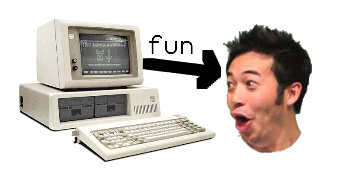
\includegraphics[width=0.5\textwidth]{use-case-dia}
  \captionsetup{justification=centering}
  \captionof{figure}{A use case diagram.  Video game (left) administering fun
                     to a user (right)}\label{fun}
\end{center}

\begin{center}
  \centering
    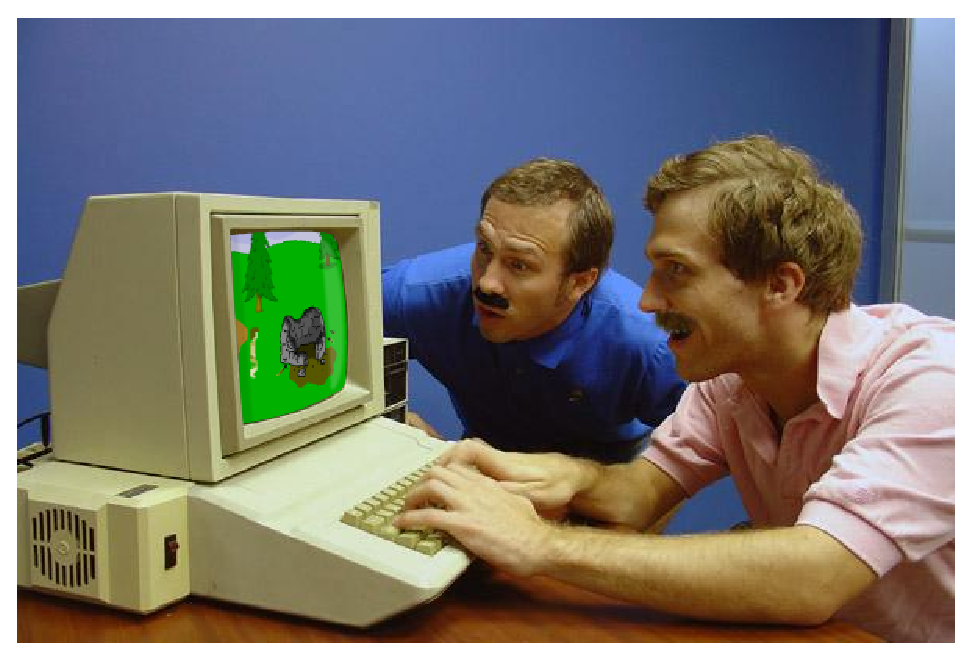
\includegraphics[width=0.5\textwidth]{Videlectrix_developers}
  \captionsetup{justification=centering}
  \captionof{figure}{The Videlectrix developers hard at work.}\label{vid-devs}
\end{center}

\clearpage

\section{Development Methodology}
As mentioned earlier, \textsf{tdm} has been implemented with
dynamically-allocated, polymorphic objects, but what does that actually mean?
Consider the two parts of the following statement.  Dynamic memory allocation in
conventional C++ parlance means that rather than building software using
variables that hold or point to data of a predetermined, fixed-size, memory can
be allocated at runtime \parencite{dymem-tut}.  This allows one to allocate
memory of a size only known at runtime, like in the following example that
allocates a variable-length \textsf{int} array of a user-specified
size\footnote{The following example is run in CERN's
excellent\footnote{} Cling LLVM-powered C++ REPL/shell
\parencite{cling,cling-news}}\footnotetext[2]{Citation needed.}:

\begin{framed}
\begin{lstlisting}[language=C++]
[cling]$ #include <iostream>
[cling]$ int *some_numbers;
[cling]$ int size = 0;
[cling]$ std::cout << "How many numbers? "; std::cin >> how_many;
How many numbers? 12
[cling]$ some_numbers = new int[how_many];
[cling]$ std::cout << "Enter " << how_many << " number" \
[cling]$           << ((how_many > 1) ? "s:" : ":") << '\n';
Enter 12 numbers:
[cling]$ for (int i = 0; i < size; i++) {
[cling]$ ?   std::cout << '#' << (i + 1) << ": ";
[cling]$ ?   std::cin >> some_numbers[i];
[cling]$ ?   }
#1: 22
#2: -27
#3: 33
#4: 12
#5: 33
#6: 23
#7: 23
#8: 23
#9: 23
#10: 23
#11: 23
#12: 23
[cling]$
\end{lstlisting}
\end{framed}

You can free the memory allocated in the above example by using the
\textsf{delete[ ]}
operator \parencite{dymem-tut}.  You can see an obvious use of this style of
memory allocation strategy in \textsf{tdm}'s \textsf{src/main.cpp}'s
\textsf{main()}'s first glance, albeit in a somewhat simpler way:

\begin{framed}
\begin{lstlisting}[language=C++]
int main(void) {
  Game *game;
  bool play_again = true;

  while (play_again) {
    game = new Game();

    play_again = game->play();

    // DELETED!!!
    delete game;
  }

  return 0;
}
\end{lstlisting}
\end{framed}


In addition to being used in allocating memory of arbitrary sizes determined
at runtime, the dynamic memory facilities in C++ can also be utilized to enable
an oft-used superpower: the ability to allocate object memory belonging to a
derived class on a pointer of its abstract base class's type.  This allows one
to store any number of \textsf{class}es and/or \textsf{struct}s in a single
data structure, so long as they are derived from the same base class.  This is 
what is referred to in C++ (and in many other
object-oriented programming\parencite{digms} languages) as \textbf{polymorphism}
\parencite{poly-tut}: the end result of combining the power of dynamic memory
allocation with the power of inheritance
inheritance\parencite{inh-g4g}.  Polymorphism can be leveraged to write code
that is powerful and concise without being overly repetitious.

In \textsf{tdm}, the above C++ development strategies ended up being used quite
heavily.  The game is primarily made up of three classes, the \textsf{Game}
class, the \textsf{Room} class, and the \textsf{Item} class:
\begin{singlespace}
\begin{framed}
\begin{lstlisting}[language=C++]
class Game {
  friend void Trinket::itm_give(void);
  friend bool Trinket::itm_get(void);
  friend void Room::parseCmd(vector<string> &args);
  friend void MainRoom::setupRoomMaps(void);
  friend void NorthRoom::setupRoomMaps(void);
  friend void SouthRoom::setupRoomMaps(void);
  friend void DennisRoom::setupRoomMaps(void);

  public:
    Game();
    ~Game();

    inline vector<string> getArgs(const string prompt);
    inline void sayArgs(vector<string> &args) const;
    inline void sayArgs(vector<string> &args, int start) const;
    inline void sayArgs(vector<string> &args,
                        int start, int end) const;
    void sayCmd(int cmd) const;
    void sayCmd(int cmd, vector<string> &args) const;
    void sayTxt(const string *_txt) const;
    void sayTxt(const string *_txt, vector<string> &args) const;
    inline void sayAnA(vector<string> &args) const;
    int getScore() const;

    void lc(string &io);

    bool play(void);

    void addToScore(int amt);
    void Over();


  private:
    void win(void);

    int score;
    bool over = false;
    bool won = false;
    bool has_trinket = false;
    Trinket *trinket;

    vector<Room *> rooms = {
      new MainRoom(), new NorthRoom(), new SouthRoom(),
      new DennisRoom()
    };

    Room *room;  // Current room

    const string txt[15] = { /* Lots of text */ };
};

class Room: public GameWumpus {
  public:
    ~Room();

    void setupItemWumpii(void);
    virtual void setupRoomMaps(void);

    virtual void desc();
    virtual void enter();  // Allows setup of room-entering events

    bool getItem(string key);
    void lookItem(string key);

    void parseCmd(vector<string> &args);

  protected:
    unordered_map<string, Item*> items;
    string room_desc;
    unordered_map<string, Room*> valid_rooms;
};

class Item : public GameWumpus {
  public:
    virtual bool itm_get(void) = 0;
    virtual void itm_look(void);
    virtual void itm_give(void);

    int getIdx(char ikey) const;
    bool getOof() const;

  protected:
    int get_idx = 0;
    int look_idx = 0;
    bool oof = false;

    vector<string> get_txt;
    vector<string> look_txt;
};
\end{lstlisting}
\end{framed}
\end{singlespace}

The \textsf{Room} and \textsf{Item} classes are abstract base classes that are
used as the basis for all of the \textsf{Game}'s various \textsf{Room}s and all
of the \textsf{Room}s' various \textsf{Item}s.  The \textsf{MainRoom},
\textsf{NorthRoom}, \textsf{SouthRoom}, and \textsf{DennisRoom} are rooms that
override \textsf{setupRoomMaps}, \textsf{desc}, \textsf{enter}, among other
things.  The \textsf{virtual} functions \textsf{void Room::desc()} and
\textsf{void Room::desc()} are overridden in the \textsf{SouthRoom} class to
account for special occasionally insulting messages the game tells the player
while there.  The \textsf{Item} class serves as the basis of the \textsf{Scroll},
\textsf{Flask}, \textsf{Parapets}, \textsf{Rope}, \textsf{Trinket}, and
\textsf{Jimberjam} classes.  Most of the \textsf{Item}s override
\textsf{itm\_get} and \textsf{itm\_look}.  For example, in the \textsf{Rope}
class:

\begin{framed}
\begin{lstlisting}[language=C++]
void Rope::itm_look(void) { game->sayTxt(&look_txt[look_idx]); }

bool Rope::itm_get(void) {
  game->addToScore(-1);
  game->sayTxt(&get_txt[get_idx]);
  game->Over();

  return false;
}
\end{lstlisting}
\end{framed}

The \textsf{Trinket} class also overrides \textsf{itm\_give}:

\begin{framed}
\begin{lstlisting}[language=C++]
void Trinket::itm_give(void) {
  if (game->room == game->rooms.at(DENNIS)) {
    string give_txt = DEN_GIVE_TKT;
    game->sayTxt(&give_txt);
    game->win();
    game->Over();
  } else {
    game->sayCmd(UNKNOWN);
  }
}
\end{lstlisting}
\end{framed}

A casual
read through the source code will reveal a quite a few uses of polymorphism, from the
\textsf{Game} class, all the way to the innermost derived \textsf{Item} classes
that live within the various intermediary \textsf{Room} classes by reference as
the \textsf{Room*} values within a \textsf{std::unordered\_map<string, Room*>},
named \textsf{items}.  The various \textsf{Room} classes themselves are also
derived from a base \textsf{Room} class are stored by reference within a
\textsf{std::vector<Room *>} container named \textsf{rooms}.

The various derived \textsf{Room}s are initialized in the \textsf{Game} class
definition found in \textsf{Game.hpp}:

\begin{framed}
\begin{lstlisting}[language=C++]
class Game {
  ...
  private:
    ...
    vector<Room *> rooms = {
      new MainRoom(), new NorthRoom(), new SouthRoom(),
      new DennisRoom()
    };
   ...
};
\end{lstlisting}
\end{framed}

The \textsf{Room}s and all of their respective \textsf{Item}s each have own
\textsf{GameWumpus} (more on those later on) initialized in
\textsf{Game::Game()}:

\begin{framed}
\begin{lstlisting}[language=C++]
Game::Game() {
  ...

  for (Room *r : rooms) {
    r->gg(this);
    r->setupItemWumpii();
    r->setupRoomMaps();
  }
}
\end{lstlisting}
\end{framed}

Setting up each \textsf{Item}'s \text{GameWumpus}:

\begin{framed}
\begin{lstlisting}[language=C++]
void Room::setupItemWumpii(void) {
  for (const auto &pair : items) {
    pair.second->gg(game);
  }
}
\end{lstlisting}
\end{framed}

All of the \textsf{Item}s in a \textsf{Room} are set up in the \textsf{Room}'s
constructor.  In the \textsf{DennisRoom}, for example, its sole \textsf{Item}
(a \textsf{Jimberjam}) is added to it's \textsf{items}:

\begin{framed}
\begin{lstlisting}[language=C++]
DennisRoom::DennisRoom() {
  items["jimberjam"] = new Jimberjam();
  room_desc = DEN_DESC;
}
\end{lstlisting}
\end{framed}

The \textsf{std::unordered\_map} of valid rooms the player can travel to
(\textsf{unordered\_map<string, Room*> valid\_rooms}) is setup in
\textsf{Room::setupRoomMaps(void)}, a \textsf{virtual} function overridden in
all derived \textsf{Room}s.  They are denoted by a \textsf{string} key (useful
for the parser) whose value is the pointer to the associated \text{Room} object
that in \textsf{rooms} vector described earlier within the \textsf{Game} class.
For example, in the \textsf{MainRoom} class the valid rooms keys are filled with
their respective \textsf{Room} pointers at enumerated \textsf{vector} indicies:

\begin{framed}
\begin{lstlisting}[language=C++]
void MainRoom::setupRoomMaps(void) {
  valid_rooms["north"] = game->rooms.at(NORTH);
  valid_rooms["south"] = game->rooms.at(SOUTH);
  valid_rooms["dennis"] = game->rooms.at(DENNIS);
}
\end{lstlisting}
\end{framed}

When the game starts, the current \textsf{Room *room} is set to point to the
instance of the \textsf{MainRoom} class, and the room is \textsf{enter}ed and
\textsf{desc}ribed:

\begin{framed}
\begin{lstlisting}[language=C++]
bool Game::play(void) {
  room = rooms.at(0);
  room->enter();
  room->desc();
\end{lstlisting}
\end{framed}

The first set of \textsf{vector<string>} arguments are captured and sent to the
current \textsf{Room}'s parser (whose structure will be described later in this
paper).  This happens in a loop until the \textsf{Game}'s \textsf{bool over}
flag has been set:
\begin{framed}
\begin{lstlisting}[language=C++]
  while (!over) {
    vector<string> args = getArgs("\nWhat wouldst thou deau?\n> ");
    room->parseCmd(args);
  }
\end{lstlisting}
\end{framed}

The \textsf{Room::parseCmd(vector<string> \&args)} performs operations on the
current \textsf{Room}'s \textsf{Item}s whenever the player tries to
\textsf{LOOK} at, \textsf{GET}, or \textsf{GIVE} an \textsf{Item}.  For example,
when the player tries to \textsf{GET} something:

\begin{framed}
\begin{lstlisting}[language=C++]
        case GET_OP: {
          Item *getter = NULL;
          if (args.size() > 1) {
            unordered_map<string, bool> ye_yon = {
              {"ye", true},
              {"yon", true},
              {"thy", true},
              {"the", true},
              {"that", true},
              {"my", true},
              {"yonder", true}
            };
            if (args.size() >= 3 && ye_yon[myargs.at(1)]) {
              getter = items[myargs.at(2)];
              if (getter) {
                getter->itm_get();
              } else {
                game->sayCmd(GET);
              }
            } else if (myargs.at(1) == "dagger") {
              game->sayCmd(GET_DAGGER);
              game->addToScore(25);
            } else {
              getter = items[myargs.at(1)];
              if (getter) {
                getter->itm_get();
              } else {
                game->sayCmd(GET, args);
              }
            }
          } else {
            game->sayCmd(UNKNOWN);
          }
          break;
        }
\end{lstlisting}
\end{framed}

\subsection{About the \textsf{GameWumpus}}
Another item of note: to easily access of the state of the game and call essential
mutator methods on the core \textsf{Game} from actions triggered by \textsf{Item}s within
\textsf{Room}s in a way that didn't completely invalidate the entire application's central
design philosophy, a
hack had to be devised, one that allowed the innermost \textsf{Room}s and
\textsf{Item}s to be able to share common utility functions with the
\textsf{Game} class without awkwardly moving functionality to the
\textsf{Item} class, adding unnecessary extra complexity to the game's design in
the process.
Below is this very hack, dubbed the \textsf{GameWumpus} class:

\begin{framed}
\begin{lstlisting}[language=C++]
class GameWumpus {
  public:
    void gg(Game *);

  protected:
    Game *game;
};
\end{lstlisting}
\end{framed}

All \textsf{Room}s and \textsf{Item}s have the DNA of a \textsf{GameWumpus}
inside of them, thanks to the magic of inheritance.  After a \textsf{Room} or an
\textsf{Item} has been created, its \textsf{void gg(Game *)} method (short for
``\textbf{g}ive \textbf{g}ame'') must be called before it can be used, to
ensure full functionality.  This hack allows public attributes and commonly-used
utility methods belonging the to the main \textsf{Game} object to be
shared and used by all of the various actions triggered throughout the
codebase that need them.  Some inner \textsf{Room} and \textsf{Item} methods
need to have additional access to \textsf{private} \textsf{Game} attributes,
hence they have been declared as \textsf{friend}s\footnote{\textsf{friend} declarations are
added to C++ classes when their pals (other friendly methods) need access to
attributes and methods that are usually private. \parencite{friend-cpp}} of the
main \textsf{Game} class, making the \textsf{Game} class by far and away the
most popular of all of \textsf{tdm}'s classes [sic].

One of the more notable shared utility functions unlocked through the power of
the \textsf{GameWumpus} is \textsf{Game}'s \textsf{sayTxt} method.  This method
is responsible for dynamically interpolating the special embedded format
specifiers embedded in many of the in-game messages with useful data from the
running \textsf{Game}:

\begin{framed}
\begin{lstlisting}[language=C++]
void Game::sayTxt(const string *_txt, vector<string> &args) const {
  for (auto c = _txt->begin(); c != _txt->end(); ++c) {
    if (*c == '%') {
      switch (*++c) {
        case ('%'):
          cout << '%';
          break;
        case ('s'):
          cout << score;
          break;
        case ('A'):
          sayAnA(args);
          break;
        case ('a'):
          sayArgs(args, 1);
          break;
        case ('v'): {
          string verb = args.at(0);
          if (verb == "gimme")
            verb = "get";

          cout << verb;
          break;
        }
      }
    } else {
      putchar(*c);
    }
  }
  putchar('\n');
}
\end{lstlisting}
\end{framed}

Another honorable mention is the utility function called by the aforementioned
\textsf{Game::sayTxt()} is \textsf{Game::sayAnA()}, a method that handles
the \textsf{\%A} format specifier within game text, used for checking if the
non-existent entity that the player has foolishly tried to \textsf{TALK} to
should be mentioned in
the resultant insulting error message with an ``a'' or an ``an'' article:

\begin{framed}
\begin{lstlisting}[language=C++]
inline void Game::sayAnA(vector<string> &args) const {
  char cons_vowel = args.at(1).at(0);
  switch (cons_vowel) {
    case 'a': case 'A':
    case 'e': case 'E':
    case 'i': case 'I':
    case 'o': case 'O':
    case 'u': case 'U':
      cout << "an";
      return;
  }
  cout << 'a';
}
\end{lstlisting}
\end{framed}

\subsection{Parsing of User Input}
Thanks to abilities granted by \textsf{std::basic\_istringstream}
\parencite{iss-cpp},
the output of the interactive game prompt's \textsf{std::getline} can
iterate over space-separated arguments, to yield a
\textsf{std::vector<string>} of  the arguments, all without the need of writing code
for scanning the input character-by-character or writing code that trims any
leading or trailing whitespace from the aforementioned input (à la Perl's \textsf{chomp()}\footnote{\cite{chomp-perldoc}}):

\begin{framed}
\begin{lstlisting}[language=C++]
inline vector<string> Game::getArgs(const string prompt) {
  vector<string> args;
  string line = "";

  while (line.length() == 0) {
    cout << prompt;
    getline(cin, line);

    if (cin.eof()) {
      cout << endl;
      exit(0);
    } else if (cin.bad()) {
      cout << endl;
      exit(1);
    }
  }

  istringstream astream(line);
  while (true) {
    string arg;
    if (astream >> arg)
      args.push_back(arg);
    else
      break;
  }
  return args;
}
\end{lstlisting}
\end{framed}

Once the arguments are separated, they get handed to the great and terrible
\textsf{Room::parseCmd(vector<string> \&args)}.  Before it does any parsing,
though, it converts the list of arguments to lowercase using the
lambda-powered\footnote{Lambdas are small anonymous functions or subroutines
that can be inserted inline in scope, often producing useful output that can be
captured. \parencite{lambda-cpp}} \textsf{void Game::lc(string \&io)} from within
a range-based \textsf{for} loop \parencite{rangeloop-cpp}:

\begin{framed}
\begin{lstlisting}[language=C++]
void Game::lc(string &io) {
  transform(io.begin(), io.end(), io.begin(),
            [](unsigned char c){ return tolower(c); });
}
\end{lstlisting}
\end{framed}

\begin{framed}
\begin{lstlisting}[language=C++]
void Room::parseCmd(vector<string> &args) {
  if (args.size() < 1)
    return;

  vector<string> myargs(args);
  for (string &arg : myargs) { game->lc(arg); }
...
\end{lstlisting}
\end{framed}


Most of \textsf{tdm}'s parsing of textual user input (taken exclusively from
\textsf{STDIN}) is handled by the monolith known as \textsf{Room::parseCmd}.
Through the magic of \textsf{std::unordered\_map}s in the C++
STL\footnote{Standard Template Library},
and the relative simplicity of the source material (at least in \emph{this}
version of \emph{Thy Dungeonman} from 2004), the entire parser has been
able to be implemented with nary a regular expression in sight (as fun as those
may
be).  To parse commands, \textsf{Room::parseCmd} runs the lowercase version of
the first argument (the verb/action to perform) from the list of arguments
through an \textsf{unordered\_map} that yields an integer value pertaining to
an \textsf{enum}erationed parser opcode keys.  The integer value from
the \textsf{unordered\_map} is fed over into a switch that hands control over
to the remainder of the parsing logic that lives at the end of its conditional
jump.  All branches of the conditional jump have both the normalized lowercase
and mixed-case versions of the argument list for in scope for parsing and
display operations, respectively.  Routing commands in this fashion affords
the ability to map multiple
verbs to the same action while also giving subsequent parsing operations ample
flexibility.  Putting function pointers in the \textsf{unordered\_map} was also
considered, but it was scrapped due to the inflexibility of being forced to
implement all subsequent parsing suboperations through functions of the same
type.

Here are some snippets of the first leg of the text parser:

\begin{framed}
\begin{lstlisting}[language=C++]
  enum cmd_ops { DESC_OP = 1, DIE_OP, DANCE_OP,
                 GET_OP, GO_OP, LOOK_OP, TALK_OP,
                 GIVE_OP, SMELL_OP, SCORE_OP, PWD_OP };

  unordered_map<string, int> cmd_map = {
    {"help", DESC_OP},
    {"helpeth", DESC_OP},
    {"look", LOOK_OP},
    {"die", DIE_OP},
    {"dance", DANCE_OP},
    {"get", GET_OP},
    // lots of GET_OP aliases...
    {"talk", TALK_OP},
    {"give", GIVE_OP},
    {"smell", SMELL_OP},
    {"sniff", SMELL_OP},
    {"go", GO_OP},
    {"score", SCORE_OP},
    {"pwd", PWD_OP},
  };
\end{lstlisting}
\end{framed}

Some locations, like \textsf{DENNIS} with its navigation commands, are
special cases that must be accounted for, in order to remain faithful to the
original game:
\begin{framed}
\begin{lstlisting}[language=C++]
  if (items["jimberjam"])
    cmd_map["not"] = GO_OP;
\end{lstlisting}
\end{framed}

Down yonder is the main command-routing \textsf{switch} statement (where the
all of the magic happens):
\begin{framed}
\begin{lstlisting}[language=C++]
  {  // (Extra {} for more explicit scoping and memory alloc.)
    auto cmd_id = cmd_map[myargs.at(0)];
    if (cmd_id) {  // If the command entered is hashed...
      switch (cmd_id) {
        case LOOK_OP:
          if (args.size() == 1) {
            desc();  // Repeat the current Room's description.
          } else {
            Item *looker = items[myargs.at(1)];
            if (looker) {
              looker->itm_look();
            } else {
              game->sayCmd(LOOK);
            }
          }
          break;
        ...
      }
    } else {  // If the command entered isn't hashed...
      game->sayCmd(UNKNOWN);
    }
  }
\end{lstlisting}
\end{framed}

\section{Results}
Before the game can run, it must first be built with GNU Autotools using the
project's included configuration:

\begin{singlespace}
\begin{framed}
\begin{verbatim}~/src/cs200-poly$ autoreconf --install
~/src/cs200-poly$ ./configure
checking for a BSD-compatible install... /usr/bin/install -c
checking whether build environment is sane... yes
checking for a thread-safe mkdir -p... /usr/bin/mkdir -p
checking for gawk... gawk
checking whether make sets $(MAKE)... yes
checking whether make supports nested variables... yes
checking for gcc... gcc
checking whether the C compiler works... yes
checking for C compiler default output file name... a.out
checking for suffix of executables... 
...
~/src/cs200-poly$ make
make  all-recursive
make[1]: Entering directory '/home/anon/src/cs200-poly'
Making all in src
make[2]: Entering directory '/home/anon/src/cs200-poly/src'
g++ -DHAVE_CONFIG_H -I. -I..     -g -O2 -MT Game.o -MD -MP -MF
.deps/Game.Tpo -c -o Game.o Game.cpp
mv -f .deps/Game.Tpo .deps/Game.Po
g++ -DHAVE_CONFIG_H -I. -I..     -g -O2 -MT main.o -MD -MP -MF
.deps/main.Tpo -c -o main.o main.cpp
mv -f .deps/main.Tpo .deps/main.Po
g++ -DHAVE_CONFIG_H -I. -I..     -g -O2 -MT Item.o -MD -MP -MF
.deps/Item.Tpo -c -o Item.o Item.cpp
mv -f .deps/Item.Tpo .deps/Item.Po
g++ -DHAVE_CONFIG_H -I. -I..     -g -O2 -MT Rooms.o -MD -MP -MF
.deps/Rooms.Tpo -c -o Rooms.o Rooms.cpp
mv -f .deps/Rooms.Tpo .deps/Rooms.Po
g++  -g -O2   -o tdm Game.o main.o Item.o Rooms.o  
make[2]: Leaving directory '/home/anon/src/cs200-poly/src'
make[2]: Entering directory '/home/anon/src/cs200-poly'
make[2]: Leaving directory '/home/anon/src/cs200-poly'
make[1]: Leaving directory '/home/anon/src/cs200-poly'
\end{verbatim}
\end{framed}
\end{singlespace}

Running the compiled game:

\begin{singlespace}
\begin{framed}
\begin{verbatim}~/src/cs200-poly$ src/tdm

 "#" # # # #   #"= # # #"# #"" #"" #"# #"# #=# #"# #"#  .   .
  #  #"#  #    # # # # # # # # #"" # # # # # # #"# # # =#= =#=
  "  " "  "    ""  """ " " """ """ """ " " " " " " " "  "   "

                    /\      /\      /\
                    ||/----\||      ||
                    \_------_/      ||
                     / o  o \       ||
                     /  ||  \    o__||__o
                     / ---- \     \____/
                     /\/\/\/\       ||
                                    oo

         ~=Press the ENTER key to enter yon dungeon=~


.....................................................
.....................................................
...............  m   m   mmm   m   m  ...............
...............  "m m"  #" "#  #   #  ...............
...............   #m#   #   #  #   #  ...............
...............   "#    "#m#"  "mm"#  ...............
...............   m"                  ...............
............... ""                    ...............
.....................................................
.....................................................
.....................................................
.....................................................
.....................................................
...............   mmm    m mm   mmm   ...............
...............  "   #   #"  " #"  #  ...............
...............  m"""#   #     #""""  ...............
...............  "mm"#   #     "#mm"  ...............
.....................................................
.....................................................
.....................................................
......................"#"............................
.......................#..#.#........................
......................."..#"#.#.#....................
.........................."."..#.....................
...............................".....................
.....................................................
.#"=.....#"#.....#""......#"#..........#"#.....#...#.
.#.#.#.#.#.#.#"".#""..#"#.#.#......#=#.#"#.#"#.".#.".
.""..#.#.".".#.#."""..#.#."."......#.#.".".#.#.".".".
....."""....."""......""".........."."....."."..."...
Ye find yeself in yon dungeon.  Ye see a SCROLL.
Behind ye scroll is a FLASK.  Obvious exits are
NORTH, SOUTH, and DENNIS.

What wouldst thou deau?
>
\end{verbatim}
\end{framed}
\end{singlespace}

From this point, the rest of the game ostensibly works, though an entire
walkthrough will not be delivered in this section, so as not to spoil the entire
game for the reader.  Instead, a few noteworthy features of the game will be
highlighted in this section
% \emph{(continued on the next page)}.
% \clearpage

New \textsf{GET} verb aliases for the player to use and discover:

\begin{singlespace}
\begin{framed}
\begin{verbatim}Ye find yeself in yon dungeon.  Ye see a SCROLL.
Behind ye scroll is a FLASK.  Obvious exits are
NORTH, SOUTH, and DENNIS.

What wouldst thou deau?
> snatch yon flask
Ye cannot get ye FLASK. It is firmly bolted to a
wall which is bolted to the rest of the dungeon
which is probably bolted to a castle. Never you mind.

What wouldst thou deau?
> yeet yon flask
Ye cannot get ye FLASK. It is firmly bolted to a
wall which is bolted to the rest of the dungeon
which is probably bolted to a castle. Never you mind.
\end{verbatim}
\end{framed}
\end{singlespace}

Appropriate verb propagation to error messages that are triggered by new
\textsf{GET\_OP} aliases:

\begin{singlespace}
\begin{framed}
\begin{verbatim}What wouldst thou deau?
> take red steckled elbermung
Thou cannotst take that. Quit making stuffeth up!

What wouldst thou deau?
> grab Da Huuuuuudge
Thou cannotst grab that. Quit making stuffeth up!

What wouldst thou deau?
> gimme deep sea fangly fish
Thou cannotst get that. Quit making stuffeth up!
\end{verbatim}
\end{framed}
\end{singlespace}

% \newpage
Correct \textsf{a/an} article selection when the player attempts to
\textsf{GIVE} something that they don't have:

\begin{singlespace}
\begin{framed}
\begin{verbatim}What wouldst thou deau?
> give Ab-Abber 2000
Thou don'tst have an Ab-Abber 2000 to give. Go back to your
tiny life.

What wouldst thou deau?
> give Lappy 486 
Thou don'tst have a Lappy 486 to give. Go back to your
tiny life.
\end{verbatim}
\end{framed}
\end{singlespace}

Just like in the original Flash game, the \textsf{SOUTH} room is stateful in its
insults:

\begin{singlespace}
\begin{framed}
\begin{verbatim}What wouldst thou deau?
> go south
You head south to an enbankment. Or maybe a chasm. You
can't decide which. Anyway, ye spies a TRINKET.
Obvious exits are NORTH.

What wouldst thou deau?
> look
Ye stand yeself close to a yet-unnamed escarpment.
Nonetheless, ye spies a TRINKET. Obvious exits are
NORTH.

What wouldst thou deau?
> get trinket
Ye getsts yon TRINKET and discover it to be a bauble.
You rejoice at your good fortune. You shove the
TRINKET in your pouchel. It kinda hurts.

What wouldst thou deau?
> go north
Ye find yeself in yon dungeon.  Ye see a SCROLL.
Behind ye scroll is a FLASK.  Obvious exits are
NORTH, SOUTH, and DENNIS.

What wouldst thou deau?
> go south
Ye stand high above a canyon-like depression. Obvious
exits are NORTH.

What wouldst thou deau?
> get trinket
Sigh. The trinket is in thou pouchel. Recallest thou?

What wouldst thou deau?
> help
Thou hangeth out at an overlook. Obvious exits are
NORTH. I shouldn't have to tell ye there is no TRINKET.

What wouldst thou deau?
>
\end{verbatim}
\end{framed}
\end{singlespace}

Live game object deletion appear and new game creation appear to all work
cleanly, though the code has yet to be extensively tested with \textsf{valgrind}
or \textsf{gdb} in conjunction with a Bash/Python fuzzer, so it cannot be said
with $100\%$ confidence that it \emph{does not} leak \emph{any} memory...
With that being said, here is an example of
\textbf{Thy Dungeonman\textsuperscript{++}}'s live reload/respawn in action
(currently broken on macOS):

\begin{singlespace}
\begin{framed}
\begin{verbatim}What wouldst thou deau?
> die
That wasn't very smart. Your score was: -95.
Play again? [Y/N] y

 "#" # # # #   #"= # # #"# #"" #"" #"# #"# #=# #"# #"#  .   .
  #  #"#  #    # # # # # # # # #"" # # # # # # #"# # # =#= =#=
  "  " "  "    ""  """ " " """ """ """ " " " " " " " "  "   "

                    /\      /\      /\
                    ||/----\||      ||
                    \_------_/      ||
                     / o  o \       ||
                     /  ||  \    o__||__o
                     / ---- \     \____/
                     /\/\/\/\       ||
                                    oo

         ~=Press the ENTER key to enter yon dungeon=~


.....................................................
.....................................................
...............  m   m   mmm   m   m  ...............
...............  "m m"  #" "#  #   #  ...............
...............   #m#   #   #  #   #  ...............
...............   "#    "#m#"  "mm"#  ...............
...............   m"                  ...............
............... ""                    ...............
.....................................................
.....................................................
.....................................................
.....................................................
.....................................................
...............   mmm    m mm   mmm   ...............
...............  "   #   #"  " #"  #  ...............
...............  m"""#   #     #""""  ...............
...............  "mm"#   #     "#mm"  ...............
.....................................................
.....................................................
.....................................................
......................"#"............................
.......................#..#.#........................
......................."..#"#.#.#....................
.........................."."..#.....................
...............................".....................
.....................................................
.#"=.....#"#.....#""......#"#..........#"#.....#...#.
.#.#.#.#.#.#.#"".#""..#"#.#.#......#=#.#"#.#"#.".#.".
.""..#.#.".".#.#."""..#.#."."......#.#.".".#.#.".".".
....."""....."""......""".........."."....."."..."...
Ye find yeself in yon dungeon.  Ye see a SCROLL.
Behind ye scroll is a FLASK.  Obvious exits are
NORTH, SOUTH, and DENNIS.

What wouldst thou deau?
> 
\end{verbatim}
\end{framed}
\end{singlespace}

\section{Analysis}
After much trial and tribulation, it can still be said that you still cannot
\textsf{GET ye FLASK}, and after all that has been learned here, it should be
readily apparent that this is as it should be, nay, as it always was
\emph{meant} to be.  All joking aside, it can definitely be said that the
goals set at the onset of this project's conception were met (and perhaps even
exceeded): a native C++ port of the original Flash/ActionScript \emph{Thy
Dungeonman} has been made, written to take full advantage of the dynamic and
polymorphic features of C++, where it has been deemed logical to do so.
Thanks to the flexibility of the C++ STL's data structures and
built-in algorithms, implementing this entire text adventure game from scratch
is just a matter of forming a cohesive mental model of the game's modes of
operation and making way for sensible base classes with which to
build the rest of the game upon.  For the most part, the polymorphism and data
types given by C++ allowed the rest to fall in place, once enough of
said basic framework was put in place, and the vision of the game's
implementation only became clearer as the work continued to progress.

In closing, it can be said that this project was a resounding success: the
parser only be said to be an improvement on the original ActionScript one,
while still retaining all of the original game's charm, even managing to take
advantage of C++'s polymorphic, dynamic feature set along the way.  The seed of
a great \emph{Thy Dungeonman} port has been planted, one that can builds on
Linux, macOS, and even Windows (using MSYS2, MinGW, or Cygwin, recommended in
that order).  With the base game and parser done, the game
can go in any number of directions, so long as I can get the blessing of
\emph{Videlectrix}, aka. \emph{The Brothers Chaps}.  Perhaps one day there will
be a version of this port using \textsf{ncurses}, \emph{SDL}, or even something
more exotic involving physical hardware!

\section{Errata}
\begin{itemize}
  \item The \textsf{Game} Burninator\footnote{Trogdor? \parencite{hrw-trog}}, er, destructor is
        broken on macOS.
\end{itemize}

\printbibliography
\end{document}
